\documentclass[12pt]{scrreprt}

%% Allgemeine Hinweise
% 
% - Windows ben�tigt Pearl zum Kompilieren
% - Guter Editor "TexStudio"
% - Nicht vergessen jedes Tex Dokument auf ISO-8859-1 zu stellen
% - Kompilierreihenfolge:
%		1. Makeglossaries
%		2. Biber
%		3. PdfLaTeX
%		4. Interner PDF-Betrachter

%--------------------------------------------------------------------------
% LaTeX packages
%--------------------------------------------------------------------------
\usepackage[ngerman]{babel}		% Neue Deute Rechtschreibung
\usepackage{pdfpages}	% PDF Import
\usepackage{geometry}	% Seitenformatierung (links, rechts usw..)
\usepackage{url}	% Urls
\usepackage{ae}		% Bessere Fonts unterst�tzung
\usepackage[latin1]{inputenc}	% Lateinisch und wichtig f�r MAC
\usepackage[T1]{fontenc}	% Westeurop�ische Kodierung
\usepackage{lmodern}	% Neue deutsche Trennungsregeln, etc 
\usepackage{mathptmx}	% Schriftart (Times New Roman)
\usepackage{acronym}	% Acronyme
\usepackage[onehalfspacing]{setspace}	% Eineinhalb Zeilen Abstand
\usepackage{titlesec}	% Titel Formatierung
\usepackage{hyperref}	% Klickbare Links
\usepackage{minitoc}	% Mini Inhaltsverzeichnis nach jeder �berschrift
\usepackage[headsepline,footsepline]{scrpage2}	% Kopf und Fu�zeilen (Seitenzahl)
\usepackage{listings}	% Quellcode
\usepackage{color}	% Farben f�rs Listing
\usepackage{float}	% Bilder zentrieren
\usepackage[right]{eurosym}
\usepackage[most]{tcolorbox} % Definitionen
\usepackage[autostyle, german=quotes]{csquotes}
\usepackage[backend=biber, style=alphabetic, citestyle=alphabetic]{biblatex}
\usepackage{chngcntr}
\usepackage{caption}
\usepackage{amsmath}
\usepackage{cleveref} % Definitionen
\usepackage[nonumberlist,	% Keine Seitenzahlen anzeigen
						acronym,	% Ein Abk�rzungsverzeichnis erstellen
						toc,	% Eintr�ge im Inhaltsverzeichnis
						section]	% Im Inhaltsverzeichnis auf section-Ebene erscheinen
						{glossaries}	% Glossar

%-----------------------------------------------------------------------------
% Settings
% ********
% Anmerkung: Die meisten Kommandos wurden in der 07_Settings/Settings.tex
% 						Datei erstellt und sollten auch nur dort ver�ndert werden.
%
%-----------------------------------------------------------------------------
% !TEX root = Settings.tex

%################################################################## COMMANDS
%##################################################################
%################################################################## 

\newcommand{\backsl}{\verb|\|} % Backslash

\newcommand{\secline}{\vspace{-1.2em}	% Linie
	\par\noindent\rule{\textwidth}{0.4pt}} 

\newcommand{\emptysite}{\newpage	% Leere Seite
	\thispagestyle{empty}
	\section*{}}

% Glossarzusatz
\renewcommand{\glossarysection}[2][]{\chapter*{#1}}	

% Farbiger Punkt
\newcommand{\tikzcircle}[2][red,fill=red]{\tikz[baseline=-0.5ex]\draw[#1,radius=#2] (0,0) circle ;}

% Abbildungsverzeichnis
\newcommand{\abbildungsverzeichnis}{\newpage
	\phantomsection
	\addstarredchapter{\textbf{Abbildungsverzeichnis}}
	\listoffigures
}

% Tabellenverzeichnis
\newcommand{\tabellenverzeichnis}{\newpage
	\phantomsection
	\addstarredchapter{\textbf{Tabellenverzeichnis}}
	\listoftables
}

% Acronyme
\newcommand{\abkuerzungen}{
	% !TEX root = Acronym.tex
\newpage
\phantomsection
\addstarredchapter{\textbf{Abk�rzungsverzeichnis}}

\chapter*{\huge\textbf{Abk�rzungsverzeichnis}}
\begin{acronym}[Bash]
	\acro{BDD}{Behavior Driven Development}
	\acro{GUI}{Graphical User Interface}
	\acro{HTML}{Hypertext Markup Language}
	\acro{IDE}{Integrated Development Environment}
	\acro{QA}{Quality Assurance}
	\acro{QM}{Qualit�tsmanagement}	
\end{acronym}
}

% Glossar
\newcommand{\glossar}{
	\newpage
	\phantomsection	
	\addstarredchapter{\textbf{Glossar}} % F�gt "Glossar" zum Inhaltsverzeichnis hinzu		
	%\addcontentsline{toc}{chapter}{\textbf{Glossar}}	% F�gt "Glossar" zum Inhaltsverzeichnis hinzu
	\printglossary[style=altlist,title=Glossar]		% Glossar
	\newpage
}

% Heading Style setzen
\newcommand{\headstyle}{
	\pagestyle{scrheadings}	% Style
	\clearscrheadfoot
	\ofoot[\pagemark]{\pagemark}
	\ohead{\headmark}
	\automark[]{chapter}
	\setheadsepline{1pt}
	\setfootsepline{0pt}
}

% Heading Style setzen (Seitenzahl Rechts)
\newcommand{\headstyleright}{
	\pagestyle{scrheadings}	% Style
	\cfoot[]{}	% [plain-Seiten]{normale Seiten} 
	\ofoot[\pagemark]{\pagemark}	% Seitenzahl
	\setheadsepline{0pt}
	\setfootsepline{0pt}
}

\newcommand{\inhaltsverzeichnis}{
	\cleardoublepage\pdfbookmark{\contentsname}{toc}
	\tableofcontents
	\clearpage
	\newpage
}

\newcommand{\literaturverzeichnis}{
	\phantomsection
	\addcontentsline{toc}{chapter}{Literatur}	% �berschrift
	\printbibliography	
}

\newcommand{\anhangstart}{
	\newpage
	%\pagenumbering{arabic}	% Arabische Ziffern
	
	\renewcommand\appendix{\par 
		\setcounter{section}{0}% 
		\setcounter{subsection}{0}% 
		\setcounter{figure}{0}% 
		
		\renewcommand\thesection{\Alph{section}}% 
		\renewcommand\thefigure{\Alph{section}\arabic{figure}}} 
	
	\numberwithin{table}{section} 
	\numberwithin{figure}{section} 
	
	
	\appendix 
	\pagestyle{empty}
	\captionsetup{listof=false}
}

\newcommand{\roemischenummerierung}{
	\pagenumbering{Roman}
}

\newcommand{\arabischenummerierung}{
	\pagenumbering{arabic}
}

%################################################################## OTHER
%##################################################################
%################################################################## 

\titleformat{name=\chapter,numberless}[display]{\normalfont\huge\bfseries}{\titlerule}{-6,9ex}{}[\vspace{3ex}]
\titlespacing{name=\chapter,numberless}{0em}{1.0em}{0em}
\titleformat{\chapter}{\normalfont\huge\bfseries}{\thechapter}{18pt}{\Huge}[{\vspace{0,6ex}\titlerule[0.8pt]\vspace{3ex}}]
\titlespacing{\chapter}{0em}{-4.0em}{0em} % {left}{before}{after}[right]
\titleformat{\section}{\normalfont\LARGE\bfseries}{\thesection}{16pt}{\LARGE}
\titleformat{\subsection}{\normalfont\Large\bfseries}{\thesubsection}{14pt}{\Large}
\titleformat{\subsubsection}{\normalfont\large\bfseries}{\thesubsubsection}{14pt}{\large}

\addbibresource{04_Literatur/Literatur.bib}
\AtBeginDocument{\counterwithin{lstlisting}{section}}
\geometry{a4paper, left=30mm, right=25mm, bottom=25mm, top=25mm}	% Text Formatierung
% !TEX root = Glossar.tex
\makeglossaries

\newglossaryentry{venturecapital}{ 
	name=Venture-Capital, 
	description={ 
		Unter Venture Capital versteht man die Finanzierung eines nicht b�rsennotierten Unternehmens mit Eigenkapital. Dabei wird das Unternehmen in der Regel zum Zeitpunkt der Beteiligung privat gehalten. Entscheidend ist, dass das Eigentum am Unternehmen w�hrend der meisten Zeit der Beteiligung in privaten H�nden liegt \autocite{venture_capital}} 
}

\newglossaryentry{servantleader}{ 
	name=Servant Leader, 
	description={ 
		Ein Servant Leader liebt Menschen und m�chte ihnen helfen. Die Aufgabe eines Servant Leaders ist es daher, die Bed�rfnisse anderer zu ermitteln und zu versuchen, diese Bed�rfnisse zu befriedigen \autocite{servant_leadership}} 
} 

\newglossaryentry{iteration}{ 
	name=Iteration, 
	description={ 
		Eine Iteration ist eine wiederholte Durchf�hrung eines Vorgangs. Die Anzahl der Durchf�hrungen (Iterationen) steht entweder vorher fest oder richtet sich nach der Erf�llung eines Abbruchkriteriums \autocite{definition_iteration} 
	}
} 

\newglossaryentry{stakeholder}{ 
	name=Stakeholder, 
	description={ 
		Anspruchsgruppen sind alle internen und externen Personengruppen, die von den unternehmerischen T�tigkeiten gegenw�rtig oder in Zukunft direkt oder indirekt betroffen sind. Gem�� Stakeholder-Ansatz wird ihnen - zus�tzlich zu den Eigent�mern (Shareholders) - das Recht zugesprochen, ihre Interessen gegen�ber der Unternehmung geltend zu machen \autocite{definition_stakeholder}
	}
}

\newglossaryentry{trialanderror}{ 
	name=Trial and Error, 
	description={ 
		Trial and Error beschreibt einen Weg, ein Ziel zu erreichen oder ein Problem zu l�sen, indem verschiedene Methoden ausprobiert und aus Fehlern gelernt wird \autocite{definition_trialanderror}
	}
}

\newglossaryentry{governance}{ 
	name=Governance, 
	description={ 
		Die Art und Weise, wie in einem Land die Angelegenheiten der Allgemeinheit verwaltet und geregelt werden. \enquote{Governance} ist nicht \enquote{Government} gleich \enquote{Regierung}, sondern umfassender und offener \autocite{definition_governance}
	}
}

\newglossaryentry{workaround}{ 
	name=Workaround, 
	description={ 
		Ein workaround beschreibt eine M�glichkeit, ein Problem zu l�sen, oder etwas trotz des Problems zum laufen zu bekommen, ohne es vollst�ndig zu l�sen \autocite{definition_workaround}
	}
}

\newglossaryentry{coredeliverable}{ 
	name=Core Deliverable, 
	description={ 
		Ein Core Deliverable ist das zentrale Produkt oder Dienstleistung, welches einem Kunden zu Verf�gung gestellt wird \autocite{definition_deliverable}
	}
}

\newglossaryentry{cicd}{ 
	name=Continous Integration, 
	description={ 
		Continous Integration beschreibt einen Softwareentwicklungsprozess, bei dem Teammitglieder h�ufig ihre Arbeit integrieren. Bei jeder Integration wird der Stand automatisch �berpr�ft, um Integrationsfehler so schnell wie m�glich zu erkennen \autocite{definition_ci}
	}
}

\newglossaryentry{devops}{ 
	name=DevOps, 
	description={ 
		Der Begriff besteht aus Development (Dev), der den Softwareentwickler beschreibt, und Operations (Ops), was den IT-Betrieb darstellt. Aus der Kombination beider soll ein Prozessverbesserungsansatz f�r die Bereiche Softwareentwicklung und Systemadministration entstehen. Es wird eine effektivere und effizientere Zusammenarbeit der verschiedenen Bereiche angestrebt \autocite{definition_devops}
	}
}
	% Glossar IMPORT
\setlength{\parindent}{0pt}	% Keine Einr�ckung am Anfang eines Absatzes
\setcounter{biburllcpenalty}{7000}
\setcounter{biburlucpenalty}{8000}

%################################################################## LISTINGS
%##################################################################
%################################################################## 

\renewcommand{\lstlistingname}{Codebeispiel}% Listing -> Codebeispiel
\renewcommand{\lstlistlistingname}{Codeverzeichnis}% List of Listings -> Codeverzeichnis

% Default fixed font does not support bold face
\DeclareFixedFont{\ttb}{T1}{txtt}{bx}{n}{12} % for bold
\DeclareFixedFont{\ttm}{T1}{txtt}{m}{n}{12}  % for normal

% Custom colors
\definecolor{deepblue}{rgb}{0,0,0.5}
\definecolor{deepred}{rgb}{0.6,0,0}
\definecolor{deepgreen}{rgb}{0,0.5,0}
\definecolor{superlightgray}{rgb}{0.97,0.97,0.97}

% Java Style
\lstdefinestyle{java}{
	language=Java,
	basicstyle=\ttm,
	otherkeywords={this},
	breaklines=true,
	tabsize=2,
	keywordstyle=\ttb\color{deepblue},
	emph={MyClass,__init__},          % Custom highlighting
	emphstyle=\ttb\color{deepred},    % Custom highlighting style
	stringstyle=\color{deepgreen},
	frame=tb,                         % Any extra options here
	belowskip=3em,
	belowcaptionskip=1em,
	aboveskip=2em,
	abovecaptionskip=1em,
	captionpos=b,
	showstringspaces=false 
}

% Java Script Style
\lstdefinestyle{travis}{
	language=bash,
	numbers=left,
	stepnumber=5,
	firstnumber=1,
	tabsize=2,
	basicstyle=\ttm,
	breaklines=true,
	alsoletter={:},
	keywords={language:, node_js:, cache:, install:, before_script:, script:},
	keywordstyle=\ttb\color{orange},
	emph={MyClass,__init__},          % Custom highlighting
	emphstyle=\ttb\color{deepred},    % Custom highlighting style
	stringstyle=\color{deepgreen},
	frame=single,                         % Any extra options here
	backgroundcolor=\color{superlightgray},
	ndkeywords={directories:},
	ndkeywordstyle=\ttb\color{deepblue},
	belowskip=2em,
	aboveskip=2em,
	abovecaptionskip=1em,
	captionpos=b,
	showstringspaces=false 
}

% Java Script Style
\lstdefinestyle{cypress}{
	language=Java,
	numbers=left,
	stepnumber=5,
	firstnumber=1,
	tabsize=2,
	basicstyle=\ttm,
	breaklines=true,
	keywords={describe, before, beforeEach, context, it, expect, equal, cy, def},
	keywordstyle=\ttb\color{orange},
	emph={MyClass,__init__},          % Custom highlighting
	emphstyle=\ttb\color{deepred},    % Custom highlighting style
	stringstyle=\color{deepgreen},
	frame=single,                         % Any extra options here
	backgroundcolor=\color{superlightgray},
	ndkeywords={assert, break, case, catch, continue, debugger, default, delete, do, else, false, finally, for, function, if, in, instanceof, new, null, return, switch, this, throw, true, try, typeof, var, void, while, with},
	ndkeywordstyle=\ttb\color{deepblue},
	belowskip=2em,
	aboveskip=2em,
	abovecaptionskip=1em,
	captionpos=b,
	showstringspaces=false 
}

% Python Style
\lstdefinestyle{python}{
	language=python,
	numbers=left,
	basicstyle=\ttm,
	otherkeywords={self},
	keywordstyle=\ttb\color{deepblue},
	emph={MyClass,__init__},          % Custom highlighting
	emphstyle=\ttb\color{deepred},    % Custom highlighting style
	stringstyle=\color{deepgreen},
	frame=tb,                         % Any extra options here
	belowskip=3em,
	aboveskip=2em,
	abovecaptionskip=1em,
	captionpos=b,
	showstringspaces=false  
}

% Bash Style
\lstdefinestyle{bash}{
	language=bash,
	basicstyle=\ttm,
	numbers=left,
	stepnumber=5,
	firstnumber=1,
	backgroundcolor=\color{superlightgray},
	otherkeywords={},
	keywordstyle=\ttb\color{deepblue},
	emph={\$},          % Custom highlighting
	emphstyle=\ttb\color{deepred},    % Custom highlighting style
	stringstyle=\color{deepgreen},
	frame=single,                         % Any extra options here
	showstringspaces=false,
	belowskip=2em,
	aboveskip=2em,
	abovecaptionskip=1em,
	captionpos=b
}

%################################################################## DEFINITONS
%##################################################################
%################################################################## 

\newtcbtheorem[number within=chapter]{Definition}{}{
	enhanced,
	attach boxed title to top left={
		xshift=-1mm,
		yshift=-5mm,
		yshifttext=-1mm
	},
	breakable,
	top=0.5em,
	bottom=-0.5em,
	colback=white,
	colframe=black,
	fonttitle=\bfseries,
	boxed title style={
		size=small,
		colback=black,
		colframe=black,
	} 
}{def}

\newenvironment{definition}[2]{ \begin{Definition}[adjusted title=#1]{}{#2} 
		\textbf{} }{\end{Definition}}

%-----------------------------------------------------------------------------
% START OF DOCUMENT														---------------------
%-----------------------------------------------------------------------------
\begin{document}

% Deckblatt & Einverst�ndnisserkl�rung

\includepdf[pages={1}]{03_PDFs/Deckblatt.pdf}
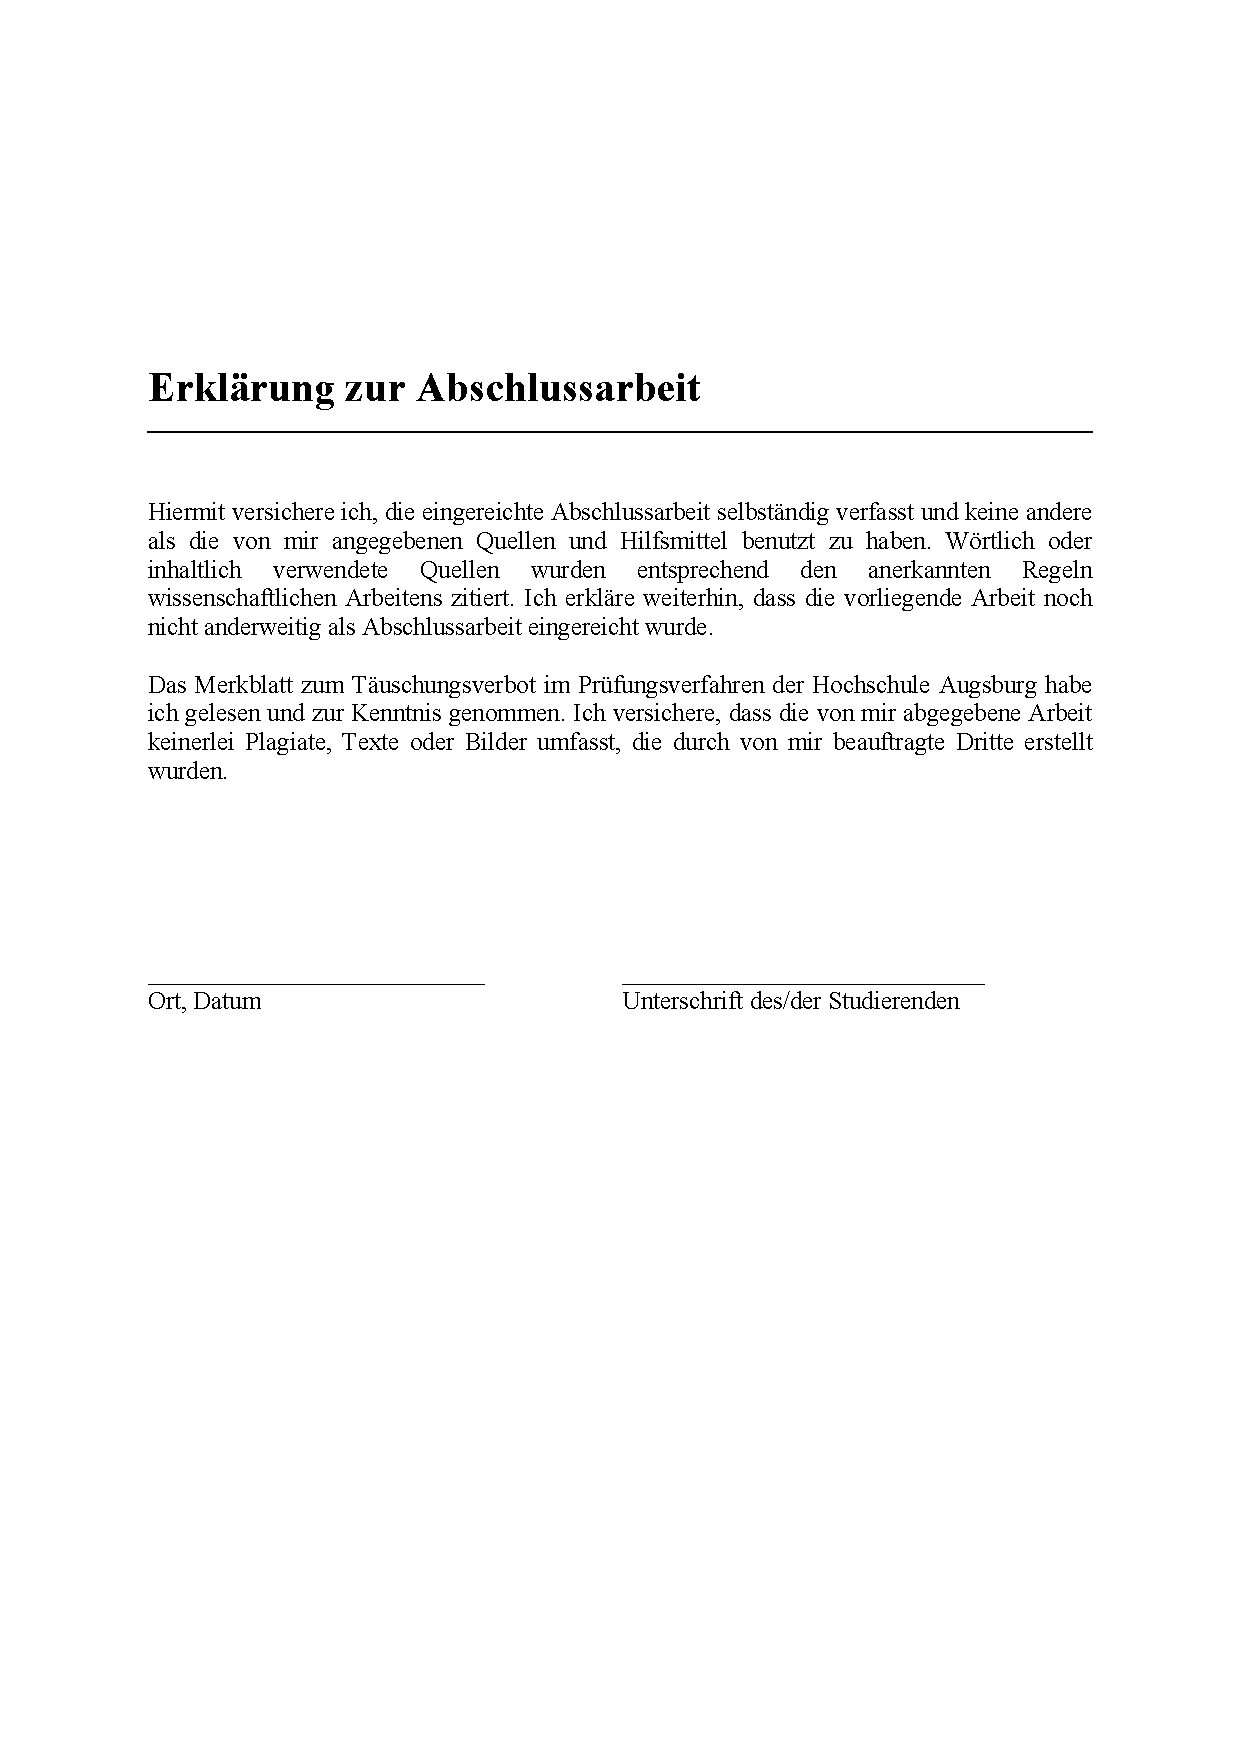
\includepdf[]{03_PDFs/Erstellungserklaerung.pdf}

% Seitenzahlformatierung (rechts)
\headstyleright

% R�mische Ziffern
\roemischenummerierung

% Setze Seitenzahl
\setcounter{page}{3}	

% Danksagung
% !TEX root = Danksagung.tex

\section*{\huge\textbf{Danksagung}}
\secline
\\\\
HIER DANKSAGUNG

\newpage


% Kurzfassung
% !TEX root = Kurzfassung.tex

\section*{\huge\textbf{Kurzfassung}}
\secline
\\\\
Viele Unternehmen sind derzeit im Umbruch in Richtung Agilit�t, obwohl diese oft die Bedeutung noch nicht genau verstehen. Agilit�t wird von einigen geliebt, von anderen nicht verstanden und vom Rest kategorisch abgelehnt. Eine Studie hat gezeigt, dass agiles Arbeiten nicht nur das Teamklima verbessert, sondern Mitarbeiter auch visions-, aufgabenorientierter und innovationsfreudiger arbeiten. Ziel dieser Arbeit ist es, herauszufinden, was genau Unternehmen davon abh�lt, von einer klassischen auf eine agile Arbeitsweise umzusteigen. Um spezifischere Ergebnisse zu erhalten, wurden diese in die drei Arten, Start-up, Mittelstand und Konzern aufgeteilt. Anschlie�end wurde ein Fragebogen erarbeitet, der das Ziel hat, Herausforderungen und Metadaten f�r die jeweiligen Unternehmensarten zu ermitteln. Neben den Ergebnissen der Frageb�gen wurden mithilfe von Erfahrungsberichten und Interviews weitere Daten erhoben. Um aus den Daten, relevante Informationen herauszufiltern, wurde die qualitative Inhaltsanalyse nach Mayring angewendet. Diese hat 45 Herausforderungen und einige Metadaten zutage gebracht. Alle Herausforderungen wurden anschlie�end aus der Sicht jeder Unternehmensart mithilfe der Metadaten bewertet. Die Bewertung hat gezeigt, dass die gr��ten Herausforderungen f�r Start-ups in der Abh�ngigkeit zu den Investoren liegen. Der Mittelstand im Vergleich ist h�ufig traditionell gepr�gt, was Herausforderungen in der Unternehmenskultur und der Verkn�pfung von IT-Systemen mit sich bringt. Dagegen liegen die Herausforderungen von Konzernen, verursacht durch die oft durchwachsene Unternehmensstruktur, oft in der Komplexit�t, der Dauer der Transformation und der damit einhergehenden hohen Kosten. Trotz der Herausforderungen muss jedes Unternehmen f�r sich entscheiden, ob es den langen Weg einer Transformation gehen m�chte. 

\newpage


% Inhaltsverzeichnis
\inhaltsverzeichnis

% Kopf und Fu�zeile
\headstyle

% Abbildungsverzeichnis
\abbildungsverzeichnis

% Tabellenverzeichnis
\tabellenverzeichnis

% Acronyme
\abkuerzungen

% Glossar
\glossar

% Arabische Ziffern
\arabischenummerierung


%-----------------------------------------------------------------------------
% HAUPTARBEIT																	HAUPTARBEIT
%-----------------------------------------------------------------------------
% !TEX root = Einleitung.tex

\chapter{Einleitung}

Jedes Projekt mit dem Ziel Software zu entwickeln, ist individuell. Aus diesem Grund gibt es in den seltensten F�llen wiederholbare Prozesse. Reproduzierbare Prozesse k�nnen durch klare Anweisungen mithilfe anschlie�ender Kontrolle befehligt oder gesteuert werden. Kreative Prozesse hingegen scheitern bei diesem Ansatz, da diese individuell, je nach Situation gesteuert werden m�ssen \autocite[vgl.][]{agiles_projektmanagement}. Um genau diese Art von Steuerung erreichen zu k�nnen, versuchen immer mehr Unternehmen einen agilen Ansatz. Diese Vorgehensweise hat das Ziel, eine kreative Probleml�sung im Team zu f�rdern, da sich Kreativit�t nicht einfach anordnen l�sst \autocite[vgl.][S.VII]{agiler_fuehren}.
\\
\begin{definition}{Definition Agile F�hrung (Quelle: \autocite{agiler_fuehren})}{def:agile_fuehrung}
	\\ 
	Agile F�hrung unterst�tzt Mitarbeiter dabei, schnell und kreativ auf wechselnde Bed�rfnisse von Kunden und M�rkten zu reagieren. Sie ist ein Mindset, eine Haltung. Sie nutzt eine offene Toolbox mit Coachingwerkzeugen, die die Zusammenarbeit verbessern, sowie Methoden zur Reduktion von Komplexit�t.
	\\
\end{definition}

Unternehmens- und F�hrungskulturen sind derzeit in vielen Unternehmen im Umbruch in Richtung Agilit�t. Bei all den Ver�nderungen in diese Richtung wissen viele Unternehmen noch nicht, was es genau bedeutet, als Unternehmen, Team oder F�hrungskraft agiler zu werden. Eine Studie (siehe \autocite[vgl.][VII]{agiler_fuehren}) mit dem Namen \enquote{Teamklima f�r Innovation} wollte herausfinden, ob sich das Teamklima in nicht-agilen Gruppen von den agilen unterscheidet. Das Ergebnis hat gezeigt, dass nicht nur das Teamklima innerhalb agil arbeitender Teams besser war, sondern diese auch visions-, aufgabenorientierter und innovationsfreudiger agieren. Zudem verbessern agile Elemente wie Visualisierung, Teamentscheidung, Retrospektive, iterative Planung und Stand-up-Meetings die Zusammenarbeit \autocite[vgl.][S.VII-VIII]{agiler_fuehren}.
\\\\ 
Das Wort \enquote{Agil} ist eine Art Reizwort, das von einigen geliebt, von anderen nicht verstanden und vom Rest kategorisch abgelehnt wird. So schrieb die amerikanische Zeitschrift \enquote{Forbes!} (siehe \autocite{managers_hate_agile}), dass Manager \enquote{agile} (Agilit�t) hassen. Die Begr�ndung der Zeitschrift f�r die Abwehrhaltung der Manager lag in einem m�glichen Machtverlust, da Agilit�t im Management gerne mit dem Abbau von F�hrung verwechselt wird. Dabei geht es gar nicht um den strikten Abbau von F�hrung, sondern eher um das F�rdern von flacheren Hierarchien. H�ufig wird die Agilit�t abgelehnt, ohne genau zu wissen, was sich dahinter verbirgt. Diejenigen, die nur eine grobe Idee davon haben, begr�nden ihre ablehnende Haltung mit dem Argument, \enquote{alle machen, was sie wollen} und bef�rchten, dass das konzernweite Chaos ausbricht \autocite[vgl.][S.1]{agiler_fuehren}.
\\\\
Hinsichtlich der Ergebnisse der eben erw�hnten Studie (siehe \autocite[vgl.][VII]{agiler_fuehren} - Teamklima f�r Innovation) stellt sich nun die Frage, ob es nicht genau diese Eigenschaften sind, die ein \enquote{modernes} Projektmanagement in Zeiten, in denen Individualit�t so eine gro�e Rolle spielt, dabei helfen, scheitern zu verhindern. Wenn Agilit�t das Mittel ist, das die Eigenschaften liefert, die ben�tigt werden, um kreative Prozesse zu f�rdern, wieso wenden nicht alle Unternehmen agile Methodiken an? 

\section{Zielsetzung \& Hypothesenbildung} \label{Kap:Zielsetzung}
Ziel dieser Arbeit ist es, herauszufinden, welche Herausforderungen Unternehmen davon abhalten, agile Methodiken anzuwenden. Dabei stellen sich die Fragen, treffen diese Herausforderungen auf alle Unternehmensarten gleicherma�en zu und k�nnen sie �berhaupt bew�ltigt werden? Zus�tzlich zu diesen Fragen werden die folgenden Hypothesen gebildet und im sp�teren Verlauf �berpr�ft:

\begin{itemize}
	\item \textbf{Die Gr��e des Unternehmens spielt eine Rolle}\\
	Desto kleiner ein Unternehmen ist, desto leichter f�llt die agile Transformation.
	
	\item \textbf{Gr��erer Innovationsdruck bei Konzernen}\\
	Je gr��er ein Konzern ist, desto mehr Innovationsdruck hin zu agilen Prozessen ist vorhanden.
	
	\item \textbf{Kosten der agilen Transformation}\\
	Die Kosten der agilen Transformation in Unternehmen, �bersteigen den Wert des Nutzen.
	
	\item \textbf{Unternehmensweites Chaos dank anarchischer Ans�tze}\\
	Bei der Einf�hrung von agilen Prozessen bricht das unternehmensweite Chaos aus.
\end{itemize}

Um die Fragen zu beantworten und die Hypothesen zu �berpr�fen, werden anhand verschiedenster Berichte, eines Fragebogens und darauf basierenden Interviews, Herausforderungen ermittelt. Zus�tzlich zu diesen, sollen auch Metadaten f�r die verschiedenen Unternehmensarten wie etwa Start-up, Mittelstand und Konzern bestimmt werden. Das hilft dabei, Herausforderungen aus der Sicht jeder Unternehmensart zu bewerten. Nach der Bewertung wird zus�tzlich dargelegt, wie die schwerwiegendsten Herausforderungen bew�ltigt werden k�nnen. Um zun�chst zu verstehen, was �berhaupt das Wort \enquote{Agilit�t} bedeutet, wird im n�chsten Kapitel Grundlagen genauer darauf eingegangen. 




% R�mische Ziffern
\roemischenummerierung

% Setze Seitenzahl
\setcounter{page}{13}

% Literatur
\literaturverzeichnis
	
% Anhang
% !TEX root = Anhang.tex

\anhangstart

\phantomsection		
\addstarredchapter{\textbf{Anhang 1, Fragebogen}} % F�gt "Glossar" zum Inhaltsverzeichnis hinzu	
\chapter*{Anhang 1, Fragebogen}

% Abbildung
\begin{figure}[H]
	\centering
	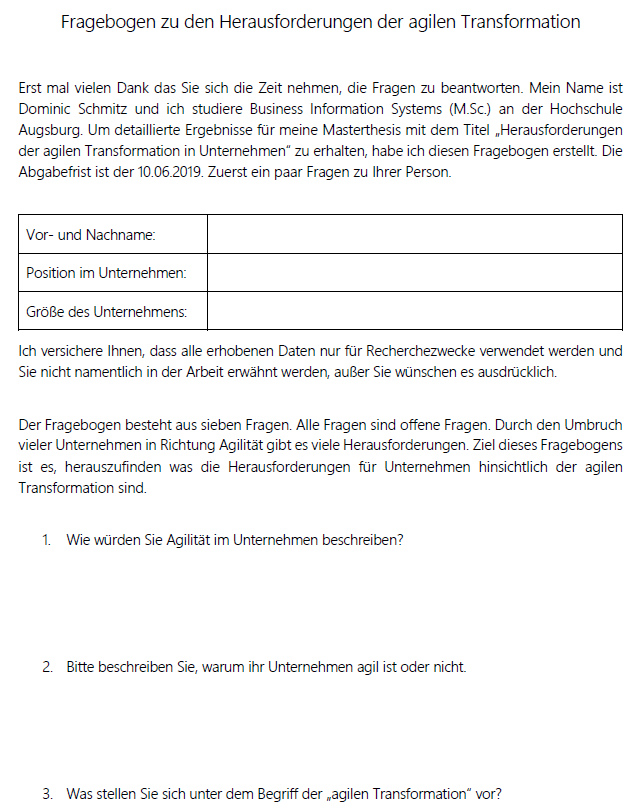
\includegraphics[width=1.0\textwidth]{06_Bilder/Fragebogen_s1.png}
	\setlength{\abovecaptionskip}{1em}
	\caption[]{Fragebogen Seite 1}
	\label{img:anh:fragebogen_s1}
\end{figure}

% Abbildung
\begin{figure}[H]
	\centering
	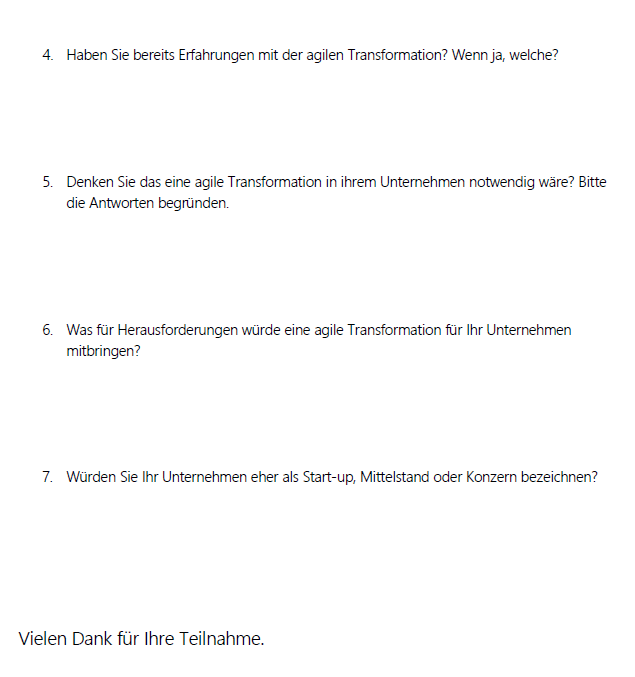
\includegraphics[width=1.0\textwidth]{06_Bilder/Fragebogen_s2.png}
	\setlength{\abovecaptionskip}{1em}
	\caption[]{Fragebogen Seite 2}
	\label{img:anh:fragebogen_s2}
\end{figure}

\phantomsection		
\addstarredchapter{\textbf{Anhang 2, Fragebogen Antworten}} % F�gt "Glossar" zum Inhaltsverzeichnis hinzu	
\chapter*{Anhang 2, Fragebogen Antworten} \label{anh:fragebogen}

\section{Antworten}

\begin{table}[H]
	\centering
	\begin{tabular}{|p{6cm}|p{8cm}|}
		\hline
		\textbf{Position im Unternehmen:}	& Gesch�ftsf�hrer	\\ \hline
		\textbf{Gr��e des Unternehmens:}	& 80 MA 			\\ \hline
	\end{tabular}
	
	\caption{Daten}
	\label{tbl:anh:antw1}
\end{table}

\begin{enumerate}
	\item \textbf{Wie w�rden Sie Agilit�t im Unternehmen beschreiben?}\\
	Agilit�t im Unternehmen bedeutet in erster Linie, dass man als Unternehmen sowie alle Abteilungen und Teams im Einzelnen schnell und unkompliziert auf die sich st�ndig �ndernden �u�eren Faktoren entsprechend reagieren k�nnen. Reagieren hei�t an dieser Stelle nicht \enquote{Dagegenhalten}, sondern diese annehmen und sich m�glichst optimal anpassen oder sogar f�r sich die maximal m�glichen Vorteile daraus ziehen. In agilen Unternehmen h�rt man den Satz \enquote{das haben wir schon immer so gemacht} immer seltener bis gar nicht. Agile Unternehmen sind etwas chaotischer strukturiert, weil nur in einem geordneten Chaos etwas Neues sich formen kann und somit dauerhaft eine Form der Ver�nderung vollzogen wird. 	
	
	\item \textbf{Bitte beschreiben Sie, warum ihr Unternehmen agil ist oder nicht.}\\
	Unser Unternehmen ist agil und soll auch weiterhin agil bleiben. Das Unternehmen geht mit jedem Projekt innovative und zum Teil neue Wege. Mit jedem Projekt, ob es am Ende erfolgreich war oder nicht, gewinnen Mitarbeiter an wertvolle Erfahrung, an neuen Methoden, an neuen Ideen. Es gibt keine feste Teamgrenzen, wir arbeiten vielmehr in virtuellen Teams, die sich auf die Herausforderung jedes Projektes einstellen und neu entstehen. Auch neue Technologien oder neue Methoden werden in unserem Unternehmen nicht nur angenommen, sondern aktiv angewendet und an unsere Kunden weitergegeben. Welche Faktoren sprechen eindeutig daf�r, dass unser Unternehmen agil ist:
	
	\begin{itemize}
		\item Wir haben OKRs eingef�hrt und arbeiten aktiv nach OKR-Modell
		\item Wir haben eine Clean Desk Policy im Unternehmen
		\item Unsere Hierarchien sind sehr flach
		\item Wir sprechen von ?One Team? in dem 80 Mitarbeiter agil arbeiten
		\item Wir erweitern unser Portfolio st�ndig mit neuen Themen
		\item Wir bitten dem Kunden nicht nur das, was wir k�nnen, sondern alles, was wir in der kurzen Zeit vor dem Projektstart noch schaffen zu lernen
		\item Wir haben eine hohe Fehlerkultur, denn nur wer etwas Neues probiert f�llt �fters auf die Nase
		\item Ein GF oder Senior Consultant arbeitet in Projekten auch mit einem Praktikanten zusammen und macht die Sch***-Aufgaben auch alleine 
	\end{itemize}
	
	\item \textbf{Was stellen Sie sich unter dem Begriff der \enquote{agilen Transformation} vor?}\\
	Agile Transformation bedeutet eine dauerhafte Ver�nderung, die sich immer wieder vorsetzt. Eine solche Transformation kann nicht abgeschlossen werden. Sie hat gewisse Etappen, die man erreichen kann, die man auch erreichen muss, aber es geht dann gleich weiter. Es ist eine st�ndige unternehmerische Weiterentwicklung, die gleichzeitig eine Verbesserung ist. Man kann an dieser Stelle sogar von kontinuierlichen Verbesserungsprozessen in einer Organisation sprechen, die zusammengefasst und aus der Flugh�he betrachtet eine agile Transformation des Unternehmens darstellen.
	
	\item \textbf{Haben Sie bereits Erfahrungen mit der agilen Transformation? Wenn ja, welche?}\\
	Fast jeder gr��ere CRM-Ansatz bedeutet eine digitale Transformation, eine neue Art zu arbeiten, mobil zu sein. Solche Projekte werden nicht nur nach agilen Methoden abgearbeitet, sondern legen Grundsteine oder sogar erreichen Etappenziele einer unternehmerischen Transformation. Ob es die gro�e SAFe- oder die kleine SCRUM- Methodik ist, unterscheidet sich die Vorgehensweise im Kern kaum. Mit SAFe wird lediglich die SCRUM-Methodik durch die Skalierung angepasst und sehr breit angewendet. Die Treiber der digitalen Transformation sind in erster Linie die IT-lastige Bereiche eines Unternehmens. F�r die Fachbereiche bedeutet die Transformation gleichzeitig einen Change, daher spielt das Change-Management w�hrend der Transformation eine entscheidende Rolle. Meine Erfahrungen mit der agilen Transformation sind vielseitig, von Neustrukturierung und dadurch Modernisierung der Unternehmensbereiche bis zu IT-Transformation von On-Demand in die Cloud. Dabei arbeiten Gro�konzerne eher nach SAFe-Methodik w�hrend die Mittelst�ndler und Kleinunternehmen von SCRUM sprechen. 
	
	\item \textbf{Denken Sie das eine agile Transformation in ihrem Unternehmen notwendig w�re? Bitte die Antwort begr�nden.}\\
	Ja, diese ist nicht nur notwendig, sondern es ist jedem im Unternehmen Bewusst, dass sich permanent vieles ver�ndern muss, um \enquote{am Ball zu blieben} und dem Mittbewerber immer \enquote{einen Schritt voraus} zu sein. Ob die Ver�nderung in der IT-Landschaft, in der Zusammenarbeit, in der Team-Zusammenstellung oder neue Standorte und neue Themenfelder ? all diese Ver�nderungen geh�ren in unserem Unternehmen zum Alltag und werden von allen Mitarbeitern nicht nur angenommen, sondern auch aktiv mitgestaltet. Wir sind mitten in einer Transformation, mal mehr agil, mal weniger, aber diese Transformation bestimmt unser Arbeitsalltag. Den unsere Kunden erwarten von uns eine Vorbildrolle, was die Digitalisierung angeht, denn wir beraten Sie zu diesen Themen, helfen den Kunden Ihre Herausforderungen in der digitalen Transformation zu schaffen. Denn die Beratungsh�user und Digitale Agenturen sind Pioniere und zugleich die Umsetzer der digitalen Transformation in der Wirtschaft.
	
	\item \textbf{Was f�r Herausforderungen w�rde eine agile Transformation f�r Ihr Unternehmen mitbringen?}\\
	Herausforderungen in folgenden Bereichen:
	\begin{itemize}
		\item \textbf{Interne Organisation:} Durch die stetig wechselnden Projektteams und Themen�berschneidungen ist es schwierig eine interne Organisation so zu fixieren, dass diese zumindest 1-2 Jahre gleich bleibt. Die Herausforderung ist dabei, nach Au�en eine klare Struktur zu zeigen und nach ihnen diese in den Griff zu bekommen ohne klare Grenzen ziehen zu m�ssen.
		
		\item \textbf{Technische Vielfalt:} Die Transformation bring viele technische Tools mit sich, die sinnvoll sind und Mehrwert liefern. Dabei muss man sehr stark aufpassen, dass man sich nicht nur noch mit der Technik besch�ftigt, die einen �berrollt und bereits morgen immer veraltet sein wird egal wie neu diese heute ist. Denn die Transformation bedeutet nicht nur technische Ver�nderung, sondern vielmehr neue Wege gehen, sich immer wieder neu ausrichten, st�ndiges Change Management zu betreiben, neue Methoden auszuprobieren, diese zu Optimieren und neue zu erfinden. Die Technik ist nur Zweck zum Erreichen des Ziels. 
		
		\item \textbf{Den Fokus zu behalten:} Mit st�ndiger Ver�nderung und Neuerung kommt die Gefahr, dass man den Fokus verliert, dass man vergisst, warum man auf dem Markt ist, warum man diese Firma gegr�ndet hat und was man mit der Firma vorhat. Man sollte die gro�en Trends beobachten, sich damit besch�ftigen, aber nicht das gesamte Gesch�ft darauf fokussieren.
		
		\item \textbf{Strategisch zu denken und eine Vision zu haben:} Herausforderung ist dabei, nicht aktionistisch zu handeln, weil es schnell sein muss, sondern strategisch �berlegt. 
		
		\item \textbf{Passende Mitarbeiter zu finden:} Denn nicht jeder mag eine st�ndige Ver�nderung, eine schnelle Entwicklung, Agilit�t in der Arbeit, Vorreiter zu sein. Ein gro�er Teil der in Frage kommenden Mitarbeiter w�rde zwar gerne mitmachen und findet Agilit�t super, aber wenn es dann darauf ankommt, will man 9to5-Job haben und einen festen Arbeitsplatz mit dem Bildrahmen der eigenen Katze auf dem Tisch. Das ist nicht agil, es ist keine Transformation. Das ist SIEMENS-Style bzw. Beamten-Style. 
		
	\end{itemize}
	
	\item \textbf{W�rden Sie Ihr Unternehmen eher als Start-up, Mittelstand oder Konzern bezeichnen?}\\
	Ich w�rde unser Unternehmen noch als Start-up bezeichnen, der auf einem guten Weg zu einem soliden Mittelstand ist. 

\end{enumerate}

\newpage

\section{Antworten}

\begin{table}[H]
	\centering
	\begin{tabular}{|p{6cm}|p{8cm}|}
		\hline
		\textbf{Position im Unternehmen:}	& Spezialist Test Management	\\ \hline
		\textbf{Gr��e des Unternehmens:}	& 200 MA 			\\ \hline
	\end{tabular}
	
	\caption{Daten}
	\label{tbl:anh:antw2}
\end{table}

\begin{enumerate}
	\item \textbf{Wie w�rden Sie Agilit�t im Unternehmen beschreiben?}\\
	Agilit�t bedeutet Verantwortung f�r das eigene Handeln zu �bernehmen sowie Freir�ume und Flexibilit�t f�r die L�sung von Problemstellungen so zu nutzen, dass das bestm�gliche Ergebnis f�r das Unternehmen entsteht.	
	
	\item \textbf{Bitte beschreiben Sie, warum ihr Unternehmen agil ist oder nicht.}\\ 
	Mein Unternehmen ist intern bereits sehr agil, da flache Hierarchien bestehen. Au�erdem sind Teams vorhanden, die nach Scrum und Kanban arbeiten sowie Konfliktmanagementprozesse, die es auf verschiedenen Stufen erm�glichen, Konflikte mit neutralen Kollegen in 1:1 Gespr�chen oder im Team zu l�sen. Dar�ber hinaus kann sich jeder einzelne Kollege einbringen und wird auch geh�rt. In der Zusammenarbeit mit externen Partnern sind wir weniger agil unterwegs, da viele externe Kollegen sehr an Hierarchien glauben und nicht selber Verantwortung f�r das eigene Handeln �bernehmen wollen. Hier ist noch die Denke vertreten: \enquote{Ich mache das, was man mir sagt, dann bekomme ich mein Geld}. Wir versuchen die Leute nun nach und nach weiter zu entwickeln, um auch da wirklich agil zu werde.
	
	\item \textbf{Was stellen Sie sich unter dem Begriff der \enquote{agilen Transformation} vor?}\\
	Agile Transformation ist f�r mich der Weg von einem hierarchischen Betriebsmodell hin zu einem agilen Unternehmen. Dieser Weg ist f�r jedes Unternehmen individuell und muss entsprechend geplant werden, damit alle Mitarbeiter abgeholt werden k�nnen.
	
	\item \textbf{Haben Sie bereits Erfahrungen mit der agilen Transformation? Wenn ja, welche?}\\
	Ja, habe ich. In verschiedenen Unternehmen war ich bei der Planung von Workshops beteiligt oder habe als QA, PO und Scrum Master agile Teams mit aufgebaut. Die Transformationen waren nicht immer leicht, da es besonders darauf ankommt Kollegen zu haben, die offen f�r die Transformation sind. Verschlie�t sich jemand, ist es oftmals unm�glich die Leute zu �berzeugen und sie verlassen �ber kurz oder lang das Unternehmen.
	
	\newpage
	\item \textbf{Denken Sie das eine agile Transformation in ihrem Unternehmen notwendig w�re? Bitte die Antwort begr�nden.}\\
	Die Transformation ist bei uns in Gange und wird auch nie abgeschlossen sein, da man sich immer weiterentwickeln und verbessern kann.
	
	\item \textbf{Was f�r Herausforderungen w�rde eine agile Transformation f�r Ihr Unternehmen mitbringen?}\\
	\begin{itemize}
		\item Externe Mitarbeiter mit eingliedern 
		\item Gegner �berzeugen
		\item Mitarbeiter enabeln Verantwortung zu �bernehmen 
		\item Zusammenarbeit mit dem Mutterkonzern, der noch sehr nach Wasserfall-lastig arbeitet
	\end{itemize}
	
	\item \textbf{W�rden Sie Ihr Unternehmen eher als Start-up, Mittelstand oder Konzern bezeichnen?}\\
	Wir sind der agile Part eines Konzerns
	
\end{enumerate}

\newpage

\section{Antworten}

\begin{table}[H]
	\centering
	\begin{tabular}{|p{6cm}|p{8cm}|}
		\hline
		\textbf{Position im Unternehmen:}	& 	VP Product Strategy\\ \hline
		\textbf{Gr��e des Unternehmens:}	& 	50 MA		\\ \hline
	\end{tabular}
	
	\caption{Daten}
	\label{tbl:anh:antw3}
\end{table}

\begin{enumerate}
	\item \textbf{Wie w�rden Sie Agilit�t im Unternehmen beschreiben?}\\
	\enquote{Agile} geht Hand in Hand mit anderen Konzepten wie \enquote{Lean} und \enquote{Management 3.0}. In meinen Augen ist es vor allem ein Wertesystem und ein Werkzeugkasten. Die Werte sind den Anforderungen einer modernen, digitalen Arbeits- und Gesch�ftswelt angepasst. Aus dem Werkzeugkasten kann man sich bedienen um eine f�r das eigene Unternehmen passenden L�sung zu schaffen. Agilit�t besteht nicht nur aus Prozessen und Workflows, die man kopieren/lernen kann.
	\\\\
	Agilit�t bottom-up einzuf�hren funktioniert aus meiner Erfahrung nicht ? top-down aber auch nicht, wenn das Executive-Management glaubt, dass das ohne Ver�nderungen f�r sie selber m�glich ist oder nicht an die zugrunde liegenden Werte  und Benefits glaubt.
	\\\\
	Es gibt kein Blueprint, es gibt nicht sowas wie \enquote{das Spotify-Modell}. Man kann \enquote{Agilit�t} einem Unternehmen nicht \enquote{verordnen}, durch Consultants beibringen. Man committet sich auf die Werte ? durch alle Managementlevel - und kann sich Unterst�tzung holen den Werkzeugkasten richtig einzusetzen.
	\\\\
	Der Gedanke vom \enquote{lernenden Unternehmen}, das sich permanent weiterentwickelt und der Ver�nderungen anpasst, wird sehr oft au�en vor gelassen/vergessen.
	\\\\
	Agilit�t betrifft alle Aspekte eines Unternehmens ? von der Organisationsstruktur bis zum Zielsystem. Sie ist nichts, was nur \enquote{in der Technik} oder ausschlie�lich in Entwicklungsteams stattfindet. Transformationen, die nur eine Abteilung im Unternehmen betreffen, scheitern schnell.
	\\\\
	Agilit�t wird auch gerne mit \enquote{chaotisch} oder \enquote{ich darf doch als Manager jeden Tag meine Meinung �ndern, oder?} verwechselt.
	\\\\
	Ein sehr h�ufiges Problem ist auch der verbliebene Wunsch nach langfristiger Milestone-Planung, der mit Agilit�t nicht vereinbar ist bzw. den die Agile Welt als nicht sinnvoll darstellt.
		
	
	\item \textbf{Bitte beschreiben Sie, warum ihr Unternehmen agil ist oder nicht.}\\
	Die Bandbreite ist hoch: einzelne Teams arbeiten agiler als andere. Einige Elemente aus dem agilen Werkzeugkasten sind umgesetzt ? aber viele auch nicht. Agile wird nicht durch das gesamte Unternehmen und alle Hierarchieebenen gelebt. Die dem \enquote{Agile} Gedanken zugrundeliegende Werte und Benefits werden aber auch nicht vollst�ndig als valide gesehen.
	\\\\
	Bei Einzelpersonen gibt es auch eine gewisse \enquote{Agile M�digkeit}: Ver�nderungsversuche aus der Vergangenheit, die nicht erfolgreich waren (aus unterschiedlichen Gr�nden), werden der Grundidee angelastet ? dadurch wird zu Weile eher polemisch �ber \enquote{Agile} gesprochen, vor allem im Senior/Executive Management (die klassischer Weise den meisten \enquote{Machtverlust} erleiden, wenn man ein Unternehmen voll und ganz Agile f�hren will).
	\\\\
	Insgesamt ist die Agilit�t f�r ein konzern-nahes Unternehmen vermutlich gar nicht so schlecht, aber gemessen an Digital Champions oder Start-ups sehr bescheiden. Das liegt IMHO vor allem daran, dass das Management nicht an die Ideen und Werte glaubt ? oder nicht bereit ist in die Transformation zu investieren bzw. den damit verbundenen Machtverlust zu akzeptieren.
	
	\item \textbf{Was stellen Sie sich unter dem Begriff der \enquote{agilen Transformation} vor?}\\
	Ich mag den Begriff nicht sehr. F�r mich schwingt da mit, dass man die Mitarbeiter umformt und sie dann nach Projektabschluss am Ziel sind.
	\\\\
	Die Werkzeuge der Agile Community entwickeln sind permanent weiter.
	Ohne mich zu sehr wiederholen zu wollen: man sollte sich auf die Werte committen und die Weichen stellen ein lernendes Unternehmen zu werden ? dann kann man eigentlich dauerhaft die notwendigen Ver�nderungen vornehmen, ohne das man jemals komplett am Ziel ist. Ver�nderung als Dauerzustand.
	
	\item \textbf{Haben Sie bereits Erfahrungen mit der agilen Transformation? Wenn ja, welche?}\\
	Ja, viele. Von Ans�tzen auf der Teamebene, der Abteilungsebene (beides bottom-up), bis zur unternehmensweiten Mission. Wenige allerdings mit nachhaltigen und guten Erfolgen. Zumeist ist es an den Dingen gescheitert, die ich bereits in den vorherigen Antwortet erw�hnt habe.
	\\\\
	Zwischenzeitlich war ich sogar hauptverantwortlich (\enquote{Chief Agile Coach}) f�r die agile Unternehmenskultur und Ver�nderung. Obwohl ich sehr leidenschaftlich an manche der agilen Ideen glaube, habe ich diese Aufgabe am Ende abgegeben ? weil es einfach zu frustierend war in der Umsetzung. Ich habe mir auch vorgenommen ? obwohl ich in dem Bereich einige Erfahrung habe ? nur dann noch mal in einer �hnlichen Rolle in einem anderen Unternehmen t�tig zu werden, wenn ich 100\% davon �berzeugt bin, dass die Unternehmensf�hrung die Konzepte versteht und hinter den Werten steht.
	
	\item \textbf{Denken Sie das eine agile Transformation in ihrem Unternehmen notwendig w�re? Bitte die Antwort begr�nden.}\\
	Ja, ich glaube nach wie vor daran, dass das Unternehmen von mehr \enquote{richtiger} Agilit�t profitieren w�rde: bessere Zusammenarbeit �ber alle Abteilungen, mehr Transparenz; mehr F�higkeit schnell auf den Markt zu reagieren; Ideen schneller austesten und verwerfen, wenn sie nicht genug Potential beweisen, ...
	
	\item \textbf{Was f�r Herausforderungen w�rde eine agile Transformation f�r Ihr Unternehmen mitbringen?}\\
	\begin{itemize}
		\item Nachdem wir in einen Konzern eingebettet sind: Strukturen au�erhalb des Unternehmens, an den Schnittpunkten zum (nicht-agilen) Konzern kompatible zur eigenen Agilit�t machen
		\item Lehre und �berzeugungsarbeit im Senior-Management (Machtverlust kompensieren/akzeptieren)
		\item Wir sitzen an zwei Standorten, bei dem einer auch noch in einem anderen Kulturkreis ist (Ukraine); alle Mitarbeiter mitzunehmen, die agilen Werte zu vermitteln, ist eine nicht zu untersch�tzende Herausforderung
		\item Das Investment der Transformation und die damit verbundenen kurzfristigen Abstriche in der Produktivit�t zu Gunsten der mittel- bis langfristigen Vorteile akzeptieren
	\end{itemize}
	
	\item \textbf{W�rden Sie Ihr Unternehmen eher als Start-up, Mittelstand oder Konzern bezeichnen?}\\
	Hybrid: Start-up like (�hnliche Herausforderungen, partiell Autonomie eines Start-ups), aber eng eingebettet in einen Konzern; Mitarbeiter-Struktur, HR-Themen sind sehr Konzern-nah.
	
\end{enumerate}

\newpage

\section{Antworten}

\begin{table}[H]
	\centering
	\begin{tabular}{|p{6cm}|p{8cm}|}
		\hline
		\textbf{Position im Unternehmen:}	& 	\\ \hline
		\textbf{Gr��e des Unternehmens:}	& 			\\ \hline
	\end{tabular}
	
	\caption{Daten}
	\label{tbl:anh:antw4}
\end{table}

\begin{enumerate}
	\item \textbf{Wie w�rden Sie Agilit�t im Unternehmen beschreiben?}\\	
	
	\item \textbf{Bitte beschreiben Sie, warum ihr Unternehmen agil ist oder nicht.}\\ 
	
	\item \textbf{Was stellen Sie sich unter dem Begriff der \enquote{agilen Transformation} vor?}\\
	
	\item \textbf{Haben Sie bereits Erfahrungen mit der agilen Transformation? Wenn ja, welche?}\\
	
	\item \textbf{Denken Sie das eine agile Transformation in ihrem Unternehmen notwendig w�re? Bitte die Antwort begr�nden.}\\
	
	\item \textbf{Was f�r Herausforderungen w�rde eine agile Transformation f�r Ihr Unternehmen mitbringen?}\\
	
	\item \textbf{W�rden Sie Ihr Unternehmen eher als Start-up, Mittelstand oder Konzern bezeichnen?}\\
	
\end{enumerate}

\newpage

\section{Antworten}

\begin{table}[H]
	\centering
	\begin{tabular}{|p{6cm}|p{8cm}|}
		\hline
		\textbf{Position im Unternehmen:}	& 	\\ \hline
		\textbf{Gr��e des Unternehmens:}	& 			\\ \hline
	\end{tabular}
	
	\caption{Daten}
	\label{tbl:anh:antw5}
\end{table}

\begin{enumerate}
	\item \textbf{Wie w�rden Sie Agilit�t im Unternehmen beschreiben?}\\	
	
	\item \textbf{Bitte beschreiben Sie, warum ihr Unternehmen agil ist oder nicht.}\\ 
	
	\item \textbf{Was stellen Sie sich unter dem Begriff der \enquote{agilen Transformation} vor?}\\
	
	\item \textbf{Haben Sie bereits Erfahrungen mit der agilen Transformation? Wenn ja, welche?}\\
	
	\item \textbf{Denken Sie das eine agile Transformation in ihrem Unternehmen notwendig w�re? Bitte die Antwort begr�nden.}\\
	
	\item \textbf{Was f�r Herausforderungen w�rde eine agile Transformation f�r Ihr Unternehmen mitbringen?}\\
	
	\item \textbf{W�rden Sie Ihr Unternehmen eher als Start-up, Mittelstand oder Konzern bezeichnen?}\\
	
\end{enumerate}

\chapter*{Anhang 3, Interviews}

\textbf{Anmerkung: } Die hier aufgef�hrten Interviews wurden am 06.06.2019 gef�hrt. Die Befragung wurde von Herrn Dominic Schmitz (Autor dieser Arbeit) gef�hrt. Die komplette Befragung wird als .mp3 Datei, dieser Arbeit zugegeben. Folgend wird das gesprochene Wort in Text umgewandelt. Hierbei ist wichtig zu erw�hnen, dass grammatikalische Fehler im besten gewissen verbessert wurden. Dabei wird in keiner wei�e die Bedeutung des Satzes und dessen Informationen ver�ndert. Die hierbei verwendeten Fragen, beziehen sich grundlegend auf die, des Fragebogens aus Anhang \ref{anh:fragebogen}. Es kommt vor, dass zus�tzliche Fragen bez�glich einer Antwort gestellt wurden.

\section{Interview Caroline Wicks Schmitz}

\begin{table}[H]
	\centering
	\begin{tabular}{|p{6cm}|p{8cm}|}
		\hline
		\textbf{Vorname, Nachname:} 		& 	Caroline, Wicks Schmitz			\\ \hline
		\textbf{Position im Unternehmen:}	& 	Chief Financial Officer (CFO)	\\ \hline
		\textbf{Name des Unternehmens:} 	&	C. \& E. Fein GmbH				\\ \hline 
		\textbf{Gr��e des Unternehmens:}	&	ca. 950 MA / 750 Mio. Umsatz im Jahr\\ \hline
	\end{tabular}
	
	\caption{Daten}
	\label{tbl:anh:int1}
\end{table}

\begin{itemize}
	\item \textbf{Wie lautet ihr vollst�ndiger Name?}\\
	Ich hei�e Caroline Wicks Schmitz. Ich bin derzeit CFO (Chief Financial Officer) der Fein Gruppe. Das ist ein Unternehmen mit weltweit circa 950 Mitarbeiternc und einem Jahresumsatz von circa 170 Millionen Euro. 
	
	\item \textbf{Sie willigen ein, dass die Befragung und die hier erhobenen Daten f�r diese Masterthesis verwendet werden d�rfen?}\\
	Selbstverst�ndlich willige ich ein.
	
	\item \textbf{Wie w�rden Sie Agilit�t im Unternehmen beschreiben?}\\
	Grunds�tzlich ist Agilit�t f�r mich eine Methode der Projektverfolgung, die Bewegung und Innovation im Unternehmen f�rdert, im Gegensatz zum klassischen Projektmanagement, dass eher einen starren Ablauf vordefiniert. Bei Fein w�rde ich sagen, dass eher das klassische Projektmanagement verwendet wird. Es werden Meilensteine definiert die den Zielen der Sprints aus agilen Formen �hneln. Zus�tzlich wird auch eine Zielplanung durchgef�hrt und es gibt review Meetings, die nicht t�glich abgehalten werden, sondern im klassischen Sinne nach erreichen eines Meilensteins. F�r die Firma Fein sind die Produktentwicklungsprojekte sehr wichtig im Projektmanagement. Dort gibt es wirklich diesen klassisch definierten Ablauf, wie ein Produkt definiert wird. Ich denke das vielleicht eine agile Vorgehensweise in diesem Bereich mehr Innovation und Kreativit�t fordern k�nnte.
	
	\item \textbf{Sie w�rden also ihren momentanen Prozess als Iterativ bezeichnen, aber die agilen Methodiken w�ren dann doch zukunftstr�chtiger?}
	Ich denke schon, dass da etwas zu gewinnen w�re. In einer klassischen Projektentwicklungsform, gehen die Ingenieure nur Schritt f�r Schritt vor hacken ihre Listen ab. In diesem Bereich w�rde nat�rlich diese reaktive Form der Agilit�t helfen selbst�ndiges Mitdenken, Kreativit�t und Eigeninitiative zu f�rdern.
	
	\item \textbf{Bitte beschreiben Sie, warum ihr Unternehmen agil ist oder nicht.}\\ 
	Ich w�rde Fein nicht als agil beschreiben, weil man eher von oben herab dieses Management by Command and Control hat. Dadurch haben die Mitarbeiter nicht den Mut Entscheidungen selber zu treffen. Das hat zur Folge, dass die Entscheidungsfreiheit und Motivation verloren geht. Die Mitarbeiter haben auch Angst vor offenen Feedback. Oft wird der Hinweis auf Fehler noch missverstanden, da die Mitarbeiter in der Unternehmenskultur noch nicht in der Lage sind, die Vorteile von offenem Feedback zu erkennen. Zus�tzlich wirkt das normale Tagesgesch�ft dagegen. Ich denke jeder Mitarbeiter hat einen hohen Anteil an Tagesgesch�ft und die Bereichs�bergreifende Zusammenarbeit wird dadurch nicht erleichtert.
	
	\item \textbf{Was stellen Sie sich unter dem Begriff der \enquote{agilen Transformation} vor?}\\
	Also f�r mich muss erst eine Basis zur agilen Transformation vorhanden sein. Es muss die Unternehmenskultur stimmen und von ganz oben herab eine Kultur der Offenheit und des Vertrauens gefordert werden. Wenn gen�gend Kapazit�ten frei sind, m�ssten von oben herab diese agilen Werte und Prinzipien zuerst gelehrt und ge�bt werden. Hierf�r m�ssten vielleicht anfangs ein paar kleinere Projekte die nicht Bereichs�bergreifend sind abgewickelt werden. So k�nnen Mitarbeiter diese Werte und Prinzipien erst mal �ben und lernen. Wichtig dabei ist, klar die Vision des Unternehmens, also wohin will das Unternehmen und was bringt uns das ganze, zu vermitteln. 
	
	\item \textbf{W�rden Sie die agile Transformation als Prozess der abgeschlossen werden kann sehen?}\\
	Nein, ich glaube das ist immer etwas das ge�bt werden muss. Nat�rlich werden manche Mitarbeiter mehr �bung als andere haben. Zus�tzlich wird es immer neue Mitarbeiter und andere Projekte mit anderen Zielen geben. Aus diesem Grund ist f�r mich die agile Transformation ein Prozess der nicht einfach so abgeschlossen werden kann. Irgendwann wird es ins Blut �bergehen, aber das ist ein Prozess der l�nger dauern wird. 
	
	\item \textbf{Haben Sie bereits Erfahrungen mit der agilen Transformation? Wenn ja, welche?}\\
	Bei Fein wurde noch keine agile Transformation durchgef�hrt, aber es wurden bereits �hnliche Elemente eingesetzt. Verwendet hatten wir KVP, also kontinuierliche Verbesserungsprozesse, bei denen wir uns immer weiter verbessert hatten. Dieser Prozess war auch nie abgeschlossen, sondern man setzt sich immer mit der Gruppe zusammen und verbessert kontinuierlich. Das wurde allerdings von der neuen Gesch�ftsf�hrung abgeschafft, weshalb ich sagen w�rde, dass Fein nicht agil Arbeitet und auch keine ansinnen danach besitzt.
	
	\item \textbf{Also will Fein zuk�nftig nicht agil agieren?}\\
	Ich hatte es schon einmal hochgebracht, aber da habe ich einfach nur gro�e Fragezeichen bei den Leuten und der Gesch�ftsf�hrung gesehen. 
	
	\item \textbf{Denken Sie das eine agile Transformation in ihrem Unternehmen notwendig w�re? Bitte die Antwort begr�nden.}\\
	Fein ist ein Traditionsunternehmen und besitzt �ber 150 Jahre Geschichte. Wir entwickeln und produzieren Elektrowerkzeuge und besitzen eine Entwicklung mit etwa 70 bis 80 Mitarbeitern. Ich denken auf jeden Fall im Entwicklungsbereich w�re die Beweglichkeit und der permanente Wandel, die Motivation und die Kreativit�t die ein agiles Vorgehen schaffen w�rde, sehr Hilfreich innovative neue Produkte zu entwickeln. Leider sind die Voraussetzungen, die durch eine entsprechende Unternehmenskultur geschaffen werden, noch nicht vorhanden. Diese m�ssten agile Vorgehensweisen unterst�tzten bevor man anf�ngt so zu arbeiten.
	
	\item \textbf{Was f�r Herausforderungen w�rde eine agile Transformation f�r Ihr Unternehmen mitbringen?}\\
	Herausforderungen w�ren das schon viele. Als erstes muss eine entsprechende Unternehmenskultur geschaffen werden, die eine entsprechende Vorgehensweise f�rdert. Ein gro�es Thema bez�glich dessen, ist die bereichs�bergreifende Zusammenarbeit bei der ich viele Herausforderungen sehe. Ein Beispiel ist das Daily Scrum. Es w�re so gut wie unm�glich im klassischen Weg, w�hrend eines Projektablaufs, allein schon einmal pro Woche Leute zusammen zu rufen, sich eine habe Stunde zusammen zu setzen. Das ist deshalb so schwierig, da jeder Bereich seine eigenen Projekte und sein eigenes Tagesgesch�ft besitzt. Hier die notwendigen Mitarbeiter regelm��ig zusammen zu bekommen ist schon ein Problem. Wenn ich allerdings sehe, was w�chentlich alles passiert, wie viele Informationen dort weitergegeben werden und wie das Team dann zusammenwachsen w�rde, w�re das schon sehr interessant t�glich ein Meeting zu veranstalten. Aber bei uns hat die Entwicklung manchmal um die 100 Projekte gleichzeitig am laufen, wie sollen die dann 100 Daily Scrums am Tag abhalten? Das mal abgesehen von irgendwelchen Projekten, die die IT oder irgend welche anderen Abteilungen im Unternehmen gerade durchf�hren. 
	
	\item \textbf{Also gibt nur Herausforderungen hinsichtlich der Meetings und der Kultur?}\\
	Grunds�tzlich sehe ich die Herausforderungen in der Unternehmenskultur, da diese sehr traditionell Deutsch ist. Fehler werden eher verp�hnt, als das diese als Opportunity gesehen werden, irgendwas zu verbessern. Zus�tzlich m�ssten Mitarbeiter mehr Vertrauen bekommen, dass es auch OK ist Fehler zu machen. Das was hierbei gelernt wird, w�rde die Firma auch weiter bringen. Das ist aber auch noch nicht vorhanden. Ein weiterer Punkt ist der, dass viele Prozesse einfach schon festgelegt sind und der Gedanke \enquote{bis jetzt hat es immer so geklappt, warum sollten wir daran etwas �ndern} noch vorhanden ist. In Wirklichkeit klappt eigentlich nichts, da wir mit dem traditionellen Gedanken nicht die notwendigen neuen innovativen Produkte entwickeln k�nnen. 
	
	\item \textbf{W�rden Sie Ihr Unternehmen eher als Start-up, Mittelstand oder Konzern bezeichnen?}\\
	Von den Statistiken her, sind wir wahrscheinlich ein Konzern. Das liegt an der H�he des Umsatzes und der Anzahl der Mitarbeiter. Das Denken im Unternehmen, entspricht eher dem des Mittelstands. Fein ist ein familiengef�hrtes traditionelles Unternehmen. Aus diesem Grund w�rde ich es eher als eine Kombination aus beiden beschreiben. 
	
	\item \textbf{W�rden Sie behaupten das die agile Transformation dem Mittelstand schwerer f�llt als anderen Unternehmensformen?}\\
	Ich denke schon, dass die agile Transformation dem Mittelstand schwerer f�llt, da der Mittelstand hier in Deutschland, traditionell sehr erfolgreich ist. Der deutsche Mittelstand ist der Wirtschaftsmotor Deutschlands. Diese Form von Unternehmen sind h�ufig Familiengef�hrte Unternehmen, die viel Erfolg �ber die Jahre und auch gute Ergebnisse gezeigt haben. Zus�tzlich wird dieses Management by Command and Control praktiziert und die Denkweise spiegelt bis jetzt sehr stark den Gedanken: \enquote{bis jetzt hat es immer so geklappt, warum sollten wir daran etwas �ndern}. Ver�nderung bei vielen mittelst�ndischen Firmen ist schwierig. Viele Merken das es Vorteile Bringt aber es liegt einfach noch nicht in deren Genen und Blut sich auf jede neue Ver�nderung zu st�rzen. H�ufig sind sie eher passiv, warten ab und schauen was andere machen bevor sie sich selbst ver�ndern. 
	
	\item \textbf{Also w�rden Sie eher den Wandel als langsam beschreiben?}\\
	Ja, sehr konservativ, sehr vorsichtig, erst mal schauen was passiert und ob es sich hierbei um eine Modeerscheinung handelt? Wieso sollen wir Geld investieren, wenn unsere klassische Denkweise uns auch voran gebracht hat?
	
	\item \textbf{Denken Sie das Konzerne einen schnelleren Wandel durchlaufen?}\\
	Konzerne werden mehr mit neuen Methodiken konfrontiert als der Mittelstand. Sie besitzen auch mehr Kapazit�ten und besitzen vielleicht auch mehr Stakeholder und Projectowners die Interesse an einer neuen Methode h�tten und so einen Wandel voran treiben. 
\end{itemize}


\section{Interview Otto-Max Herbstritt}

\begin{table}[H]
	\centering
	\begin{tabular}{|p{6cm}|p{8cm}|}
		\hline
		\textbf{Vorname, Nachname:} 		& 	Otto-Max Herbstritt				\\ \hline
		\textbf{Position im Unternehmen:}	& 	Chief Information Officer (CIO)	\\ \hline
		\textbf{Name des Unternehmens:} 	&	C. \& E. Fein GmbH				\\ \hline 
		\textbf{Gr��e des Unternehmens:}	&	ca. 950 MA	 					\\ \hline
	\end{tabular}
	
	\caption{Daten}
	\label{tbl:anh:int2}
\end{table}

\begin{itemize}
	\item \textbf{Wie lautet ihr vollst�ndiger Name?}\\
	Otto-Max Herbstritt.
	
	\item \textbf{Wie lautet ihre aktuelle Position?}\\
	Ich bin selbst�ndig als Interims CIO.
	
	\item \textbf{Was f�r eine Position haben sie bei Fein ausge�bt?}\\
	C. \& E. Fein GmbH, Chief Information Officer (CIO).
	
	\item \textbf{Sie willigen ein das die erhobenen Daten der Befragung f�r diese Masterarbeit verwendet werden d�rfen?}\\
	Ja.
	
	\item \textbf{Wie w�rden Sie Agilit�t im Unternehmen beschreiben?}\\
	Ich kann diese Frage nur auf IT-Projekte beziehen. Bei Fein gab es erst einmal keine Agilit�t. Wir hatten ein agiles Projekt mit dem Thema der CRM Einf�hrung aber das lief aus meiner Sicht genauso wie ein normales Projekt. Die IT-Projekte wurden von mir immer bei Fein vorangetrieben, dort habe ich pers�nlich agil gehandelt. Es gab w�chentliche Meetings mit den Projektteilnehmern und Mitarbeitern und ich hab mich, sofern es notwendig war, immer mit dem Fachbereich abgestimmt. Wenn ich ein agiles Projekt im Unternehmen Fein beschreiben m�sste, kann ich das nicht, denn es gab keins. Ich pers�nlich w�rde iterativ vorgehen wenn ich agil handeln w�rde. Das was man fr�her in einem St�ck erledigt hat, wird jetzt in mehreren St�cken erledigt.
	
	\item \textbf{Bitte beschreiben Sie, warum ihr Unternehmen agil ist oder nicht.}\\
	Wie schon erw�hnt, Fein geht in der IT nicht agil vor, da die Projektzeiten eigentlich immer festgelegt wurden auf ein Jahr und in diesem Zeitraum auch abgeschlossen wurden. Im Rahmen dieses Zeitfensters gab es auch nur einen Abschluss. Zus�tzlich gab es immer gen�gend Zeit die Projekte vern�nftig zu planen mit entsprechender Luft. Des Weiteren war es auch so, dass ich gar keine Chance f�r das agilen Projektmanagement gesehen habe. Es wurden die Mitarbeiter ausgebildet, aber nicht f�r agile Herangehensweisen. Wenn dies doch der Fall ist, m�ssen alle mitmachen, nicht nur die IT-Abteilung. Aus diesen Gr�nden w�rde ich unser Unternehmen nicht als agil bezeichnen. 
	
	\item \textbf{Was stellen Sie sich unter dem Begriff der \enquote{agilen Transformation} vor?}\\
	Darunter stelle ich mir vor, dass die ganze Firma, alle Projekte agil steuert. Beispielsweise mithilfe eines Frameworks wie etwa Scrum. Um dies allerdings zu verwirklichen m�ssen alle Mitarbeiter hinreichend geschult werden. Jeder Mitarbeiter im Unternehmen muss diese Vorgehensweise auch unterst�tzten damit dies Erfolg bringt. Wenn es nicht unterst�tzt wird, und beispielsweise ein Mitarbeiter Schwierigkeiten macht, tauchen die ersten Probleme auf. Somit muss die ganze Firma darauf ausgerichtet sein, alle Mitarbeiter entsprechend geschult werden und in der Lage sein sich daf�r Zeit zu nehmen. Diese Zeit ist in vielen Unternehmen gar nicht gegeben, da das Gesamtheitliche nicht gesehen wird und jeder Mitarbeiter sein eigenes Tagesgesch�ft besitzt. Auch die Bereichs�bergreifenden Prozesse m�ssen angepasst werden und Vorgesetzte m�ssen entsprechende Konsequenzen tragen. Oft denken allerdings die Fachbereiche nicht Bereichs�bergreifend was zus�tzlich zu Problemen f�hrt. 
	
	\item \textbf{Haben Sie bereits Erfahrungen mit der agilen Transformation? Wenn ja, welche?}\\
	Nein.
	
	\item \textbf{Denken Sie das eine agile Transformation in ihrem Unternehmen notwendig w�re? Bitte die Antwort begr�nden.}\\
	Ja, ist notwendig, da Gesch�ftsprozesse oft Bereichs�bergreifend sind. Wenn nur die IT die Projekte vorantreibt und die Fachbereiche den Gedanken \enquote{Ist ja nur ein IT-Projekt} besitzen, funktioniert das nicht. Auch die Fachbereiche m�ssen mithelfen und die Kapazit�ten zur Verf�gung stellen und die Zeit daf�r aufbringen (gegeben falls Freistellen), damit gerade agile Prozesse umgesetzt werden k�nnen. Ich wei� die Frage bezieht sich auf die Transformation, allerdings w�re es schon mal sch�n einen Vergleich zwischen einem nicht agilen und agilen Projekt zu sehen.
	
	\item \textbf{Was f�r Herausforderungen w�rde eine agile Transformation f�r Ihr Unternehmen mitbringen?}\\
	Erstmal muss die Zusammenarbeit von oben nach unten verbessert werden. Das bedeutet, dass auch die Gesch�ftsf�hrung dahinter stehen muss. Sie sollte nicht nur \enquote{Br�llen} wenn etwas nicht funktioniert. 
	Vorgesetzte m�ssen akzeptieren das Mitarbeiter mehr Zeit ben�tigen. So muss das Verst�ndnis aufgebracht werden, dass weniger Zeit f�r das Tagesgesch�ft vorhanden ist, da die Aufgaben des Sprints auch erledigt werden m�ssen. Alle Mitarbeiter m�ssen auch geschult werden hinsichtlich des agilen Projektmanagements, damit sie erfahren f�r was das alles gut ist. Zus�tzlich sollte noch eine Stelle geschaffen werden, die entsprechende KPI�s hat um das zentrale Projektmanagement auch entsprechend zu managen. Diese Stelle sollte in der Lage sein zu sagen, da haben wir ein Problem, da muss gehandelt werden. Das sollte relativ neutral passieren, damit der entsprechende Business Owner in dem es das Problem gibt auch reagieren kann. 
	
	\item \textbf{W�rden Sie Ihr Unternehmen eher als Start-up, Mittelstand oder Konzern bezeichnen?}\\
	Fein ist Mittelstand. 
	
	\item \textbf{W�rden Sie behaupten das die agile Transformation dem Mittelstand schwerer f�llt als anderen Unternehmensformen?}\\
	Es kommt auf die F�hrungskultur an und wie gro� der Mittelstand ist. Wenn ich einen kleinen Mittelstand nehme, zwischen 50 und 100 Mitarbeitern f�llt es denen sicherlich schwer, weil die nicht laufend so viele Projekte machen und alle sehr Hands-on sind, da sie sonst nicht Flexibel w�ren. Der gro�e Mittelstand wie beispielsweise Fein, k�nnte es durchaus umsetzen, wenn konsequent die Gesch�ftsf�hrung auch dahinter w�re und die Mitarbeiter machen l�sst, ohne dauernd rein zu funken, wenn denen etwas nicht gef�llt. Zusammengefasst w�rde ich also behaupten das es dem kleinen Mittelstand schwerer f�llt, hingegen dem gro�en einfacher. Das liegt daran das der kleine Mittelstand pragmatischer Orientiert ist als der gro�e.
	Zus�tzlich h�ngt es nat�rlich auch von den Projekten ab und wie diese definiert sind. Wenn ein Projekt durchgef�hrt wird, sieht man es aus Unternehmenssicht strategisch, da ein Ziel erreicht werden soll. Aus Anwendersicht wird es nicht strategisch gesehen, denn dieser will einfach nur schnell sein Problem gel�st haben. Die Anwendersicht wird h�ufig im kleinen Mittelstand vertreten hingegen beim gro�en Mittelstand eher die strategische. 
	Ein weiterer Aspekt ist die Abh�ngigkeit der verschiedenen Systeme und wie diese miteinander verkn�pft sind. Fein besitzt sehr viele Systeme und automatisierte Prozesse im Vergleich zu anderen Unternehmen, was nat�rlich eine Transformation noch einmal zus�tzlich erschwert. 
	
	
\end{itemize}




%-----------------------------------------------------------------------------
% END OF DOCUMENT														  ---------------------
%-----------------------------------------------------------------------------
\end{document}

